% !Mode:: "TeX:UTF-8"
% !TEX $P_r$ogram  = xelatex
\documentclass[a4paper]{article}
\usepackage{amsmath}
\usepackage{amssymb}
\usepackage{siunitx}
\usepackage{ctex}
%\usepackage{braket}
%\usepackage[european]{circuitikz}
\usepackage{multirow}
\usepackage{float}
\usepackage{graphicx}
\usepackage{geometry}
\geometry{left=2.5cm,right=2.5cm,bottom=2.5cm,top=2.5cm}
\title{近代物理实验报告10.2:铁电薄膜铁电性能的表征}
\author{xy\quad 学号\quad 匡亚明学院}
\date{2019年2月29日}
\begin{document}
\maketitle
\bibliographystyle{unsrt}
%--------main-body------------

\section{引言}
铁电体是这样一类材料: 在一定温度范围内存在自发极化, 自发极化具有两个或多个可能的取向, 其取向可能随电场而转向。铁电体并不含“铁”,只是它与铁磁体具有磁滞回线相类似,具有电滞回线,因而称为铁电体(Ferroelectrics)。在某一温度以上,它为顺电相,无铁电性,其介电常数服从居里-外斯(Curie-Weiss)定律。铁电相与顺电相之间的转变通常称为铁电相变,该温度称为居里温度或居里点$T_c$。铁电体即使在没有外界电场作用下,内部也会出现极化,这种极化称为自发极化。自发极化的出现是与这一类材料的晶体结构有关的。

晶体的对称性可以划分为32种点群。在无中心对称的21种晶体类型种除432点群外其余20种都有压电效应,而这20种压电晶体中又有10种具热释电现象。热释电晶体是具有自发极化的晶体,但因表面电荷的抵偿作用,其极化电矩不能显示出来,只有当温度改变,电矩(即极化强度)发生变化,才能显示固有的极化,这可以通过测量一闭合回路中流动的电荷来观测。热释电就是指改变温度才能显示电极化的现象,铁电体又是热释电晶体中的一小类,其特点就是自发极化强度可因电场作用而反向,因而极化强度和电场E之间形成电滞回线是铁电体的一个主要特性。

自发极化$P_s$可用矢量来描述,在相变温度,自发极化出现在晶体中造成一个特殊的方向。每个晶胞中原子的构型使正负电荷重心沿这个特殊方向发生相对位移,使电荷正负中心不重合,形成电偶极矩。整个晶体在该方向上呈现极性,一端为正,一端为负,在其正负端分别有一层正和负的束缚电荷,这些表面束缚电荷将产生一退极化场$E_d$,它与$P_s$方向相反。束缚电荷产生的电场在晶体内部与极化方向反向,使静电能升高,在受机械约束时,伴随着自发极化的应变还将使应变能增加,所以均匀极化的状态是不稳定的。晶体将分成若干小区域,每个小区域内部电偶极子沿同一方向,但各个小区域电偶极子方向不同,这些小区域称为铁电畴或畴(domain),畴的间界叫畴壁(domain wall)。铁电畴的出现是为了降低铁电体由顺电相到铁电相相变时所带来的弹性能和静电能。但畴壁的存在引入了畴壁能。施加几十kV/cm大于矫顽场$E_c$的外场时,铁电畴将沿着外场方向排齐。总自由能取极小值的条件决定了电畴的稳定性。

铁电薄膜中的畴壁为1nm$\sim$10nm的数量级。

\section{实验目的}
\begin{enumerate}
    \item 了解什么是铁电体,什么是电滞回线及其测量原理和方法。
    \item 了解非挥发铁电随机读取存储器的工作原理及性能表征。
\end{enumerate}

\section{实验仪器}
电滞回线测量仪。

\section{实验原理}
\subsection{铁电体的特点}
\subsubsection{电滞回线}
铁电体的极化随外电场的变化而变化,但电场较强时,极化与电场之间呈非线性关系。在电场作用下新畴成核长,畴壁移动,导致极化转向,在电场很弱时,极化线性地依赖于电场(见图(\ref{fig3})OA段),此时可逆的畴壁移动成为不可逆的,极化随电场的增加比线性段快。当电场达到相应于B点值时,晶体成为单畴,极化趋于饱和。电场进一步增强时,由于感应极化的增加,总极化仍然有所增大(BC)段。如果趋于饱和后电场减小,极化将循CBD段曲线减小,以致当电场达到零时,晶体仍保留在宏观极化状态,线段OD表示的极化称为剩余极化$P_r$。将线段CB外推到与极化轴相交于E,则线段OE为饱和自发极化$P_s$。如果电场反向,极化将随之降低并改变方向,直到电场等于某一值时,极化又将趋于饱和。这一过程如曲线DFG所示,OF所代表的电场是使极化等于零的电场,称为矫顽场$E_c$。电场在正负饱和度之间循环一周时,极化与电场的关系如曲线CBDFGHC所示此曲线称为电滞回线(HysteresiSloop)。
\begin{figure}[!h]
    \begin{minipage}{0.48\textwidth}
        \begin{center}
            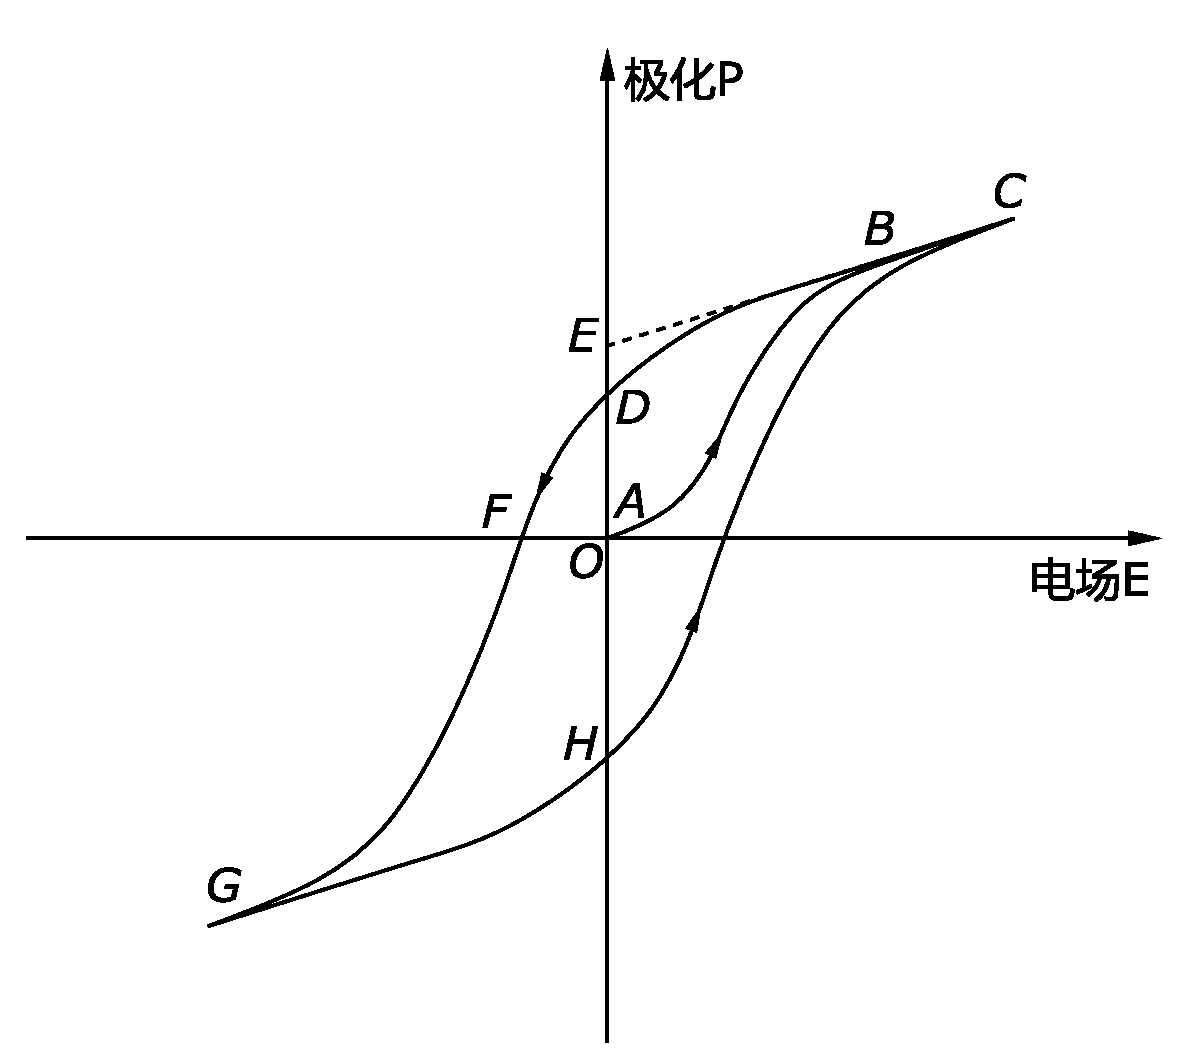
\includegraphics[width=0.95\textwidth]{fig/fig3.pdf}\\
            \caption{铁电体的电滞回线}\label{fig3}
        \end{center}
    \end{minipage}
    \begin{minipage}{0.48\textwidth}
        \begin{center}
            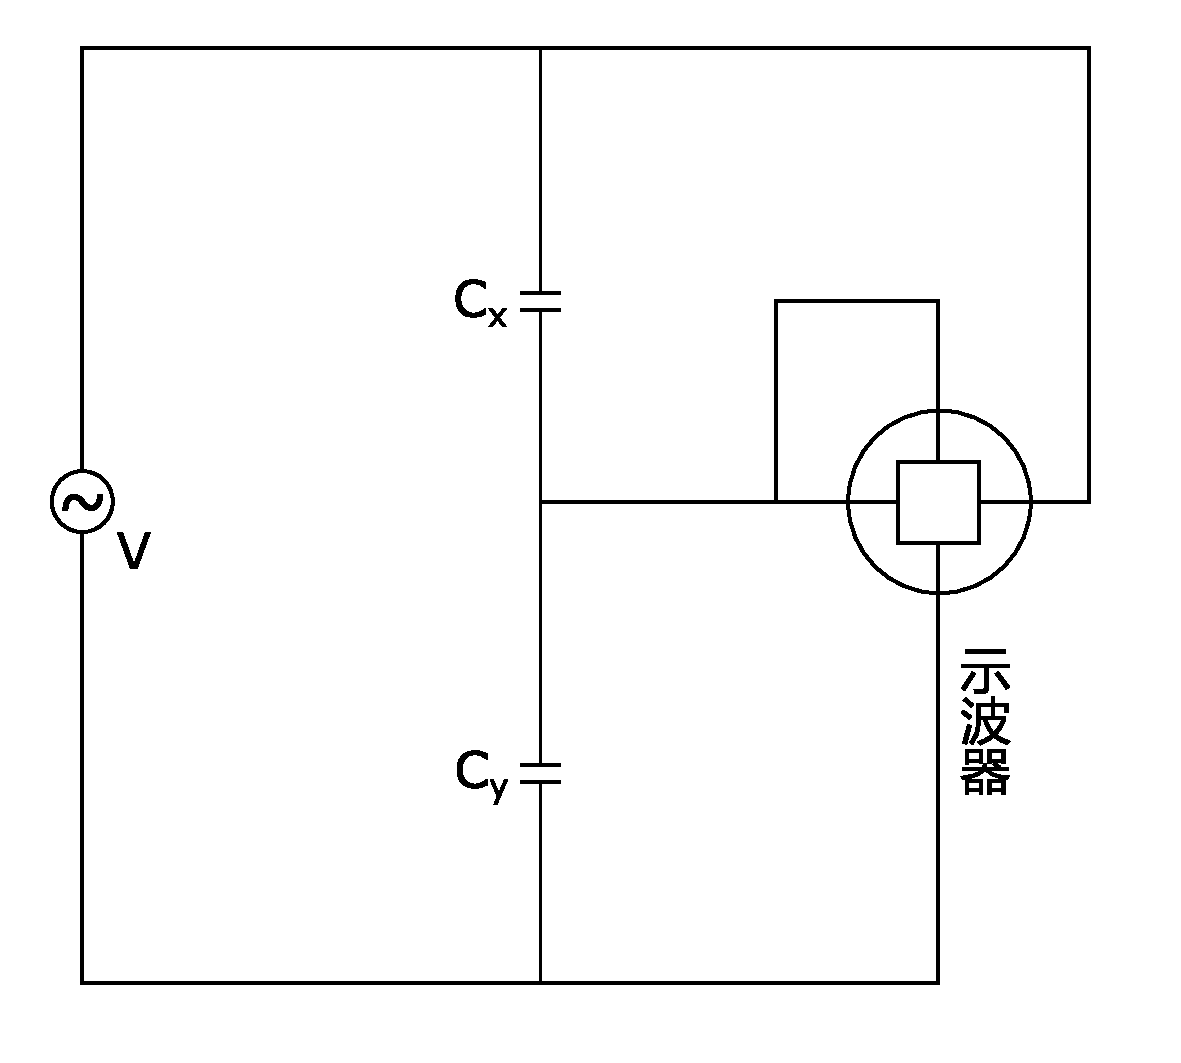
\includegraphics[width=0.95\textwidth]{fig/fig4.pdf}\\
            \caption{测量电路图}\label{fig4}
        \end{center}
    \end{minipage}
\end{figure}

电滞回线可以用图(\ref{fig4})装置显示出来(这就是著名的Sawyer-Tower电路),以电晶体作介质的电容$C_x$上的电压V是加在示波器的水平电极板上,与$C_x$串联一个恒定电容$C_y$(即普通电容),$C_y$上的电压$V_y$加在示波器的垂直电极板上,很容易证明$V_y$与铁电体的极化强度P成正比,因而示波器显示的图象,纵坐标反映P的变化,而横坐标$V_x$与加在铁电体上外电场强成正比,因而就可直接观测到P-E的电滞回线。

下面证明$V_y$和P的正比关系,因:
\begin{equation}
    \cfrac{V_y}{V_x} = \cfrac{\frac{1}{\omega C_y}}{\frac{1}{\omega C_x}} = \cfrac{C_x}{C_y}\label{eq1}
\end{equation}
式中$\omega$为图中电源V的角频率:$C_x = \epsilon\frac{\epsilon_0S}{d}$,$\epsilon$为铁电体的介电常数,$\epsilon_0$为真空的介电常数,S为平板电容$C_x$的面积,d为平行平板间距离,代入(\ref{eq1})式得:
\begin{equation}
    V_y = \cfrac{C_x}{C_y}V_x = \cfrac{\epsilon\epsilon_0S}{C_y}\cfrac{V_x}{d} = \cfrac{\epsilon\epsilon_0S}{C_y}E\label{eq2}
\end{equation}
根据电磁学:
\begin{equation}
    P = \epsilon_0(\epsilon - 1)E \approx \epsilon_0\epsilon E = \epsilon_0\xi E\label{eq3}
\end{equation}
对于铁电体$\epsilon\gg 1$,故有后一近似等式,代入(\ref{eq2})式
\begin{equation}
    V_y = \cfrac{S}{C_y}P\label{eq4}
\end{equation}
因S与$C_y$都是常数,故$V_y$与P成正比。
\subsubsection{居里点$T_c$}
当温度高于某一临界温度$T_c$时, 晶体的铁电性消失。这一温度称为铁电体的居里点。由于铁电体的消失或出现总是伴随着晶格结构的转变,所以是个相变过程,已发现铁电体存在两种相变:一级相变伴随着潜热的产生,二级相变呈现比热的突变,而无潜热发生,又铁电相中自发极化总是和电致形变联系在一起,所以铁电相的晶格结构的对称性要比非铁电相为低。如果晶体具有两个或多个铁电相时,最高的一个相变温度称为居里点,其它则称为转变温度。
\subsubsection{居里-外斯定律}
由于极化的非线性,铁电体的介电常数不是常数,而是依赖于外加电场的,一般以OA曲线(图(\ref{fig3}))在原点的斜率代表介电常数,即在测量介电常数时,所加外电场很小,铁电体在转变温度附近时,介电常数具有很大的数值,数量级达。当温度高于居里点时,介电常数随温度变化的关系为
\begin{equation}
    \epsilon = \cfrac{C}{T - T_0}+\epsilon_{\infty}\label{eq5}
\end{equation}
\subsubsection{铁电体的分类}
铁电体的分类方法很多,按其所含的基本单元的不同可划分为一下几种:
\begin{enumerate}
    \item 含氧八面体的铁电体
    \item 含氢键的铁电体
    \item 含其它离子基团的铁电体
    \item 铁电聚合物与铁电液晶
\end{enumerate}
\subsection{铁电体的应用}
铁电体具有介电、压电、热释电、铁电性质以及与之相关的电致伸缩性质、非线性光学性质、电光性质、声光性质、光折变性质、铁电记忆存储性能等等,都与其电极化性质相关,特别是电介质的热释电与铁电性质都与其自发极化相关。由于铁电体具有上述性质,因而在诸多高技术中有着很重要的应用。

利用其压电性能可制作电声换能器,用于超声波探测,声纳,稳频振谐器,声表面波器件等; 利用其热释电性质可制作红外探测器,红外监视器,热成像系统等; 利用非线性光学效应可制作激光倍频、三倍频、和频、差频器;利用电光性质可制作激光电光开关、光偏转器、光调制器等;利用声光效应可制作激光声光开关、声光偏转器、声光调制器等;利用光折变效应可制作光存储器件;而铁电材料的铁电性可制作铁电记忆存储器。
\subsection{铁电储存应用}
铁电记忆存储器(Ferroelectric Memory)是利用铁电体所具有的电滞回线性质。如图(\ref{fig3})所示,当加到铁电体上电场为零时,铁电体上仍保持有一定的极化强度$P_r$(或$-P_r$),这个极化电荷的符号取决于该电体上原加场的符号。若原来加的正场,则当外场变为零场时,铁电体上为正的剩余极化($+P_r$)而若是从负场变到零场,则此时剩余极化为负($-P_r$)。正是利用这无外场时所有的两个稳定极化$P_r$作为计算机编码0($+P_r$)和1($-P_r$),这就是铁电记忆及逻辑电路的基础。

铁电记忆存储是铁电体极少数利用铁电体的铁电性能去工作,而不是其他性能(如热电、压电、电光等)的应用。在铁电存储器应用中,即使电源突然中断,其储存的信息也可保持,因而通常称为非易失性铁电随机读取存储器(Non-Volatile Ferroelectric Random Access Memory, NV-FeRAM)。铁电体不仅作为一个电容,而且其本身也作为一个存储单元。铁电存储器由于其尺寸小(是通常可擦除随机只读存储器的20\%),抗辐照(特别适用于军用和航天使用),存储读取速度高,容易与硅工艺相容,因而有很好的前景。目前铁电随机存储器已有商品销售,由其为核心的智能卡及作为嵌入式芯片已用于众多家电的控制器如洗衣机、游戏机、电视频道存储记忆器、复印机、收费站刷卡等等方面,随大存储量的产品出现将在数码相机、随身听中使用,市场前景看好。
铁电材料的铁电性能最为重要的表征是其电滞回线所反映的铁电性能,包括饱和极化$P_s$, 永久极化$P_r$,矫顽场$E_c$等,而对于用于铁电存储器的铁电薄膜来讲,除此之外还有漏电流$I_k$,铁电疲劳性能(永久极化与开关次数关系$R_r-n$)及铁电保持性能(永久极化与时间关系$R_r-t$)。通常要求永久极化$P_r>10\mu \text{C/cm}^2$,矫顽场$E_c<100\text{kV/cm}$。好的疲劳特性,在铁电翻转10$^9$次时,永久极化很少变化。在10$^5$秒内可较好的保持电荷,漏电流小于10$^{-7}\text{A/cm}^2$
\subsection{铁电薄膜的制备方法}
铁电薄膜的制备方法多种多样,常见的大致分为两类,一类属于物理气相沉积(PVD)方法,常见的有溅射法(Sputtering)、脉冲激光沉积法(Pulsed Laser Deposition)、激光分子束外延(Laser Molecular Beam Epitaxy)等。另一类属于化学气相沉积法(CVD),常见的有金属有机源气相沉积(MOCVD)和原子层化学气相沉积(ALCVD)。此外,还有热蒸发法,湿氧化法等其它制备方法。下面简要介绍集中常见的制备方法。
\begin{enumerate}
    \item 溅射法: 常见的有磁控溅射和离子束溅射。其优点是制备薄膜的成本较低,可以制备供工业应用的大面积薄膜。薄膜的制备不仅可以使用陶瓷靶材,也可在氧气氛围中使用金属或合金靶材进行反应溅射。这种制备方法的缺点是,如果各组元的挥发性差别很大,溅射生长的薄膜成分和靶材成分将会有较大偏差,而且其偏差大小与工艺制备条件有关。
    \item 脉冲激光沉积法:PLD方法是20世纪80年代迅猛发展起来的制备薄膜技术。它利用经过聚焦而具有很高能流密度的紫外脉冲激光束瞬间融溶靶材,产生高压高能的等离子体,最终在衬底上沉积成膜。此方法的最大优点是沉积的薄膜与靶材的成分很接近,因而可以通过调控靶材的成分来严格控制薄膜成分。由于光源为能量较高的紫外脉冲激光,所以PLD能制备高熔点、多组分的氧化物薄膜和异质结构。其主要的缺点是不能制备大面积厚度均匀的薄膜。
    \item 激光分子束外延(LMBE):其基本是原理与PLD类似。其主要的优点是可在薄膜生长过程中进行原位观测,实现单原子层生长,从而获得高纯度、厚度均匀可控的超薄膜,所以特别适合用于生长外延单晶膜或多层膜。缺点是生长薄膜时需要较高真空度(<10$^{-5}$Pa),所以对仪器的要求很高。
    \item 化学气相沉积法(CVD):该方法的特点是在材料进行化学反应合成的同时成膜,其中以金属有机源气相沉积(MOCVD)的用途最广,一般工业生产用此法。这种方法的优点是可以制备大面积均匀的薄膜包括外延单晶膜,而且薄膜沉积速率调控范围很大(1nm/min$\sim$1000nm/min)。此方法的缺点是对于许多的氧化物材料而言,能适用的具有足够高饱和蒸汽压的金属有机源(简称MO源)难以合成。原子层化学气相沉积(ALCVD)能实现单原子层生长从而能制备出高质量的超薄膜,但是其技术的高要求和操作的复杂性使得其应用的普及性受到很大限制。
    \item 有机金属沉积(MOD):MOD沉积是制备铁电薄膜的最方便的技术,同时也是目前实验室使用旋涂(spin-on)技术制备铁电薄膜的方法。MOD和spin-on技术结合制备薄膜有很多优点:(1)成分均匀且易控制;(2)与MOCVD相比,退火处理后薄膜中的含碳量低;(3)工艺简单。但同时也有些不利之处,比如只能在平面上沉积薄膜、为达到所需薄膜厚度需通过多次旋涂在层间会造成高缺陷密度,易产生漏电。
    \item 凝胶法:是将金属的醇盐或其他有机盐溶解于同一溶剂中,经过水解、聚合反应形成溶胶。通过甩胶在基片上形成薄膜,经过干燥和退火处理,形成铁电薄膜。此方法能够精确控制膜的化学计量比和掺杂,易于制备大面积的薄膜,适于大批量生产,设备简单,成本低,可与微电子工艺技术相兼容。但这种方法易有不足之处,如膜的致密性较差,干燥处理过程中薄膜一出现龟裂现象,薄膜结构和生长速率对基片和电极材料很敏感。迄今为止,利用该方法已制备出PT、PZT、PLZT、BT、ST、BST等多种铁电薄膜。
\end{enumerate}

\section{实验内容}
\begin{enumerate}
    \item 通过铁电薄膜的电滞回线测量得到薄膜的永久极化$P_r$、矫顽场$E_c$, 漏电流$I_k$,这是铁电薄膜的铁电性能的表征。
          %    \item 研究铁电存储有关的性能,测量用于存储记忆的铁电薄膜的开关疲劳性能及保持性能。
\end{enumerate}

\section{实验步骤}
\begin{enumerate}
    \item 开启计算机。
    \item 阅读仪器说明书。
    \item 开启测量仪器。
    \item 检查探针位置是否正确。
    \item 测量电滞回线。
    \item 关闭测量仪。
    \item 关闭计算机。
\end{enumerate}

\newpage

\section{实验数据}
我们得到了如图(\ref{1200V}-\ref{1550V})所示的电滞回线,共15条,由于篇幅有限,仅举2例。
\begin{figure}[!h]
    \centering
    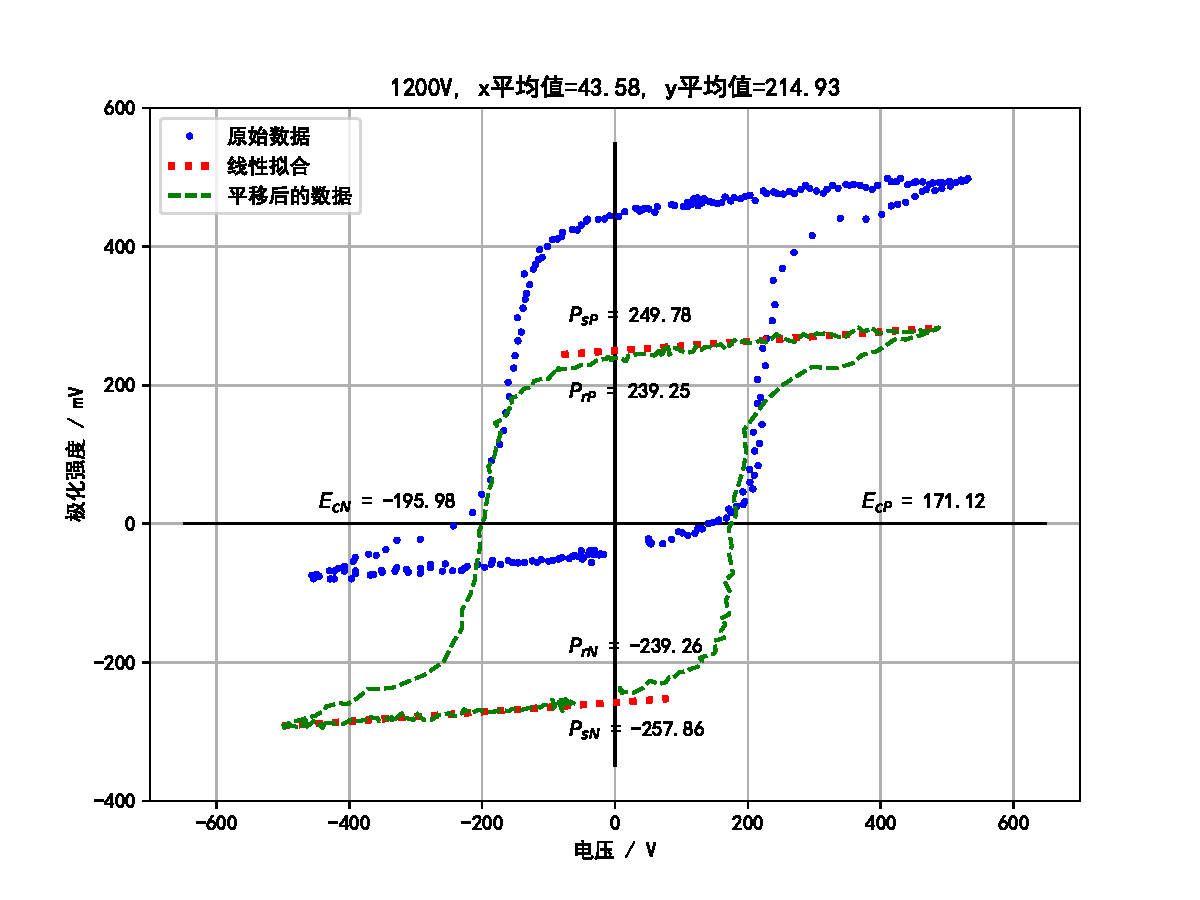
\includegraphics[width=0.82\textwidth]{fig/1200V.pdf}
    \caption{电滞回线,V=1200V}\label{1200V}
\end{figure}

\begin{figure}[!h]
    \centering
    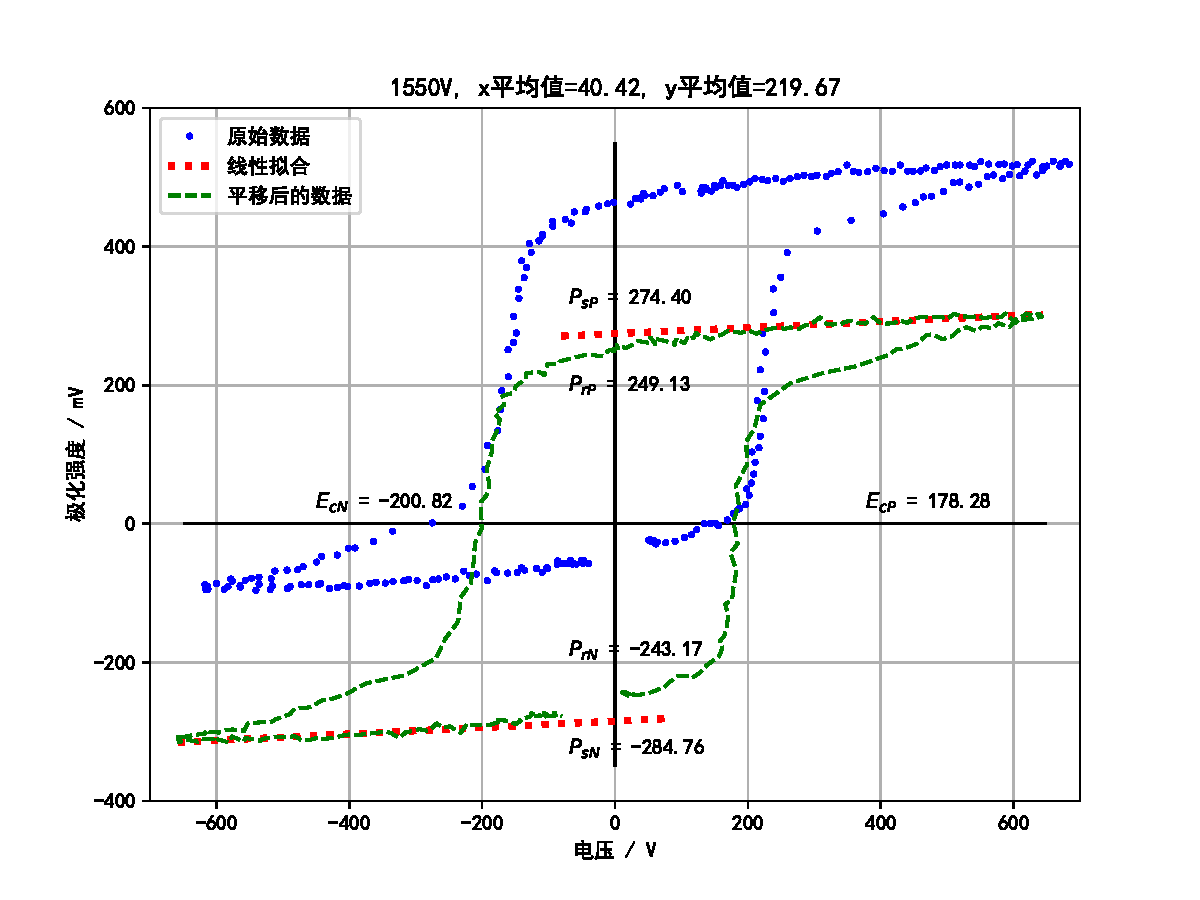
\includegraphics[width=0.82\textwidth]{fig/1550V.pdf}
    \caption{电滞回线,V=1550V}\label{1550V}
\end{figure}

其中我们对原始数据做了平移处理。我们可以看到原始数据在纵坐标上漂移较大,考虑到铁电体的电滞回线应该是对称的,我们把横纵坐标的数据都减去了对应的平均值,用修正后的数据计算所需的3对数据$E_c$、$P_r$、$P_s$。

\begin{enumerate}
    \item 取电压极大值和极小值后测量的40个数据点进行线性拟合,求出拟合直线的纵截距,作为饱和自发极化$P_s$,分别记为$P_{sP}$和$P_{sN}$;
    \item 取最靠近y轴的两个数据点的电压值作为剩余极化$P_r$,分别记为$P_{rP}$和$P_{rN}$;
    \item 取最靠近x轴的两个数据点的电压值作为矫顽场$E_c$,分别记为$E_{cP}$和$E_{cN}$。
\end{enumerate}

得到的数据如表(\ref{parameters})所示:

\begin{table}[!ht]
    \centering
    \begin{tabular}{|c|c|c|c|c|c|c|}
        \hline
        电压 / V & $E_{cP}$ / V & $E_{cN}$ / V & $P_{rP}$ / mV & $P_{rN}$ / mV & $P_{sP}$ / mV & $P_{sN}$ / mV \\ \hline
        1200     & 171.12       & -195.98      & 239.25        & -239.26       & 249.78        & -257.86       \\ \hline
        1225     & 175.03       & -195.47      & 237.24        & -238.57       & 251.44        & -258.85       \\ \hline
        1250     & 183.80       & -195.10      & 237.80        & -238.70       & 255.28        & -262.90       \\ \hline
        1275     & 177.99       & -199.31      & 243.57        & -243.03       & 254.98        & -265.29       \\ \hline
        1300     & 170.97       & -200.03      & 236.65        & -241.87       & 261.58        & -264.60       \\ \hline
        1325     & 179.13       & -198.47      & 238.16        & -243.09       & 261.58        & -264.08       \\ \hline
        1350     & 182.14       & -199.56      & 236.75        & -233.20       & 260.96        & -266.12       \\ \hline
        1375     & 182.49       & -200.21      & 245.28        & -238.02       & 260.61        & -271.41       \\ \hline
        1400     & 177.06       & -202.44      & 240.80        & -244.54       & 262.21        & -280.98       \\ \hline
        1425     & 184.05       & -191.65      & 241.22        & -235.33       & 263.47        & -278.23       \\ \hline
        1450     & 182.17       & -199.13      & 246.73        & -239.24       & 264.18        & -278.05       \\ \hline
        1475     & 180.39       & -194.61      & 246.39        & -239.49       & 267.80        & -275.90       \\ \hline
        1500     & 172.72       & -193.98      & 246.25        & -241.24       & 270.30        & -283.16       \\ \hline
        1525     & 180.97       & -198.53      & 245.67        & -242.39       & 271.76        & -276.95       \\ \hline
        1550     & 178.28       & -200.82      & 249.13        & -243.17       & 274.40        & -284.76       \\ \hline
    \end{tabular}
    \caption{15条电滞回线的3对参数}\label{parameters}
\end{table}

将表(\ref{parameters})中的数据对电压作图,可以得到3种参数随电压变化的关系,其中还增加了成对参数的平均数,如图(\ref{E_c}-\ref{P_s})所示:
\begin{figure}[!h]
    \centering
    \includegraphics[width=0.8\textwidth]{fig/E_c.pdf}
    \caption{矫顽场$E_c$与电压关系}\label{E_c}
\end{figure}

\begin{figure}[!h]
    \centering
    \includegraphics[width=0.8\textwidth]{fig/P_r.pdf}
    \caption{剩余极化$P_r$与电压关系}\label{P_r}
\end{figure}

\begin{figure}[!h]
    \centering
    \includegraphics[width=0.8\textwidth]{fig/P_s.pdf}
    \caption{饱和自发极化$P_s$与电压关系}\label{P_s}
\end{figure}

从图中可以看出,随电压增大,矫顽场缓慢增大,饱和自发极化和剩余极化都较快增大。

\newpage
\phantom{something}
\newpage

\section{实验分析和讨论}
\iffalse
\subsection{讨论3种参数与电压的关系}
在图(\ref{E_c})中我们发现数据点与线性拟合的差距较大,数据的线性不是很好。我们取样的点是电滞回线两端电压达到极值后的40个点,一开始我们只取20个点,得到的数据的线性程度比图(\ref{E_c})所示的更加差。我们认为是实验仪器的记录的电压数量较少、涨落较大造成的。另外在图(\ref{1200V})和(\ref{1550V})中也发现图象下半段缺少了一块数据,这是实验仪器本身电压范围的限制造成的,使得$P_r$的测量较为不准确。

如果需要改进,可以尝试加密实验仪器的取点数量,提高仪器的探测精确度;使仪器提供的电压能覆盖一整个回线范围。

\subsection{试比较铁电体与铁磁体的异同。}
\begin{itemize}
\item 相同之处:
\begin{enumerate}
    \item 电滞回线与磁滞回线相对应,电畴与磁畴有很大类似性。都可以用来做记忆材料。
    \item 顺电-铁电相变对应顺磁-铁磁相变,它们都有居里温度的概念,并在顺电(顺磁)的情况下满足居里-外斯定理。
\end{enumerate}
\item 不同之处:
\begin{enumerate}
    \item 铁电畴壁的厚度很薄。大约是几个晶格常数的量级,但铁磁畴壁则很厚,可达到几百个晶格常数的量级(例如对Fe,磁畴壁厚约$\SI{1000}{\angstrom}$),而且在磁畴壁中自发磁化方向可逐步改变方向,而铁电体则不可能。
    \item 铁电体在外电场作用下,自发极化的方向也只能在某几个方向中变化。但是铁磁体在足够强的外磁场作用下能够完全转到外场方向,而不论外场相对于晶轴的角度如何。
\end{enumerate}
\end{itemize}

\subsection{铁电薄膜为什么能用作数据存储器,其优点何在?}
铁电记忆存储器是利用铁电体具有的电滞回线的性质:若原来加的正场,当外场变为零的时候,铁电体上为正的剩余极化($+$),若原来加的负场,当外场变为零的时候,则剩余极化为负($-$)。因而可以进行编码,正为1,负为0。铁电存储器尺寸小、抗辐射、存取速度快且功耗低。
\fi

\nocite{jiaocai}
\bibliography{ref}
\end{document}